\documentclass{beamer}

%\setbeameroption{show only notes} % Only notes
\setbeameroption{show notes on second screen=right} % Both
%\setbeamerfont{note page}{size=\tiny}
%\setbeameroption{hide notes} % Only slides

\usepackage[utf8]{inputenc}
\usepackage[T1]{fontenc}
\usepackage{hyperref}
\usepackage{transparent}

\usetheme{ec}

\newcommand{\OPTversion}{dev-local}


\newcommand{\sepframe}[2]{
    \setbeamercolor{background canvas}{bg=ectext}

    \begin{frame}[noframenumbering,plain]
        \begin{tikzpicture}[remember picture,overlay]
            \fill[ecaccentblue] (0,0) rectangle(.05,\paperheight);
        \end{tikzpicture}
      \begin{tikzpicture}[remember picture,overlay]
          \ifx\insertframesubtitle\@empty%
              {\node[anchor=west, ecaccentblue, font=\huge] at (0,.25){\uppercase\expandafter{#1}};}
          \else%
              {
                  \node[anchor= west, ecaccentblue, font=\huge] at (0,.25){\uppercase\expandafter{#1}};%
                  \node[anchor= west, white,font=\small] at (0,-.5){\uppercase\expandafter{#2}};}%
          \fi
      \end{tikzpicture}

      \begin{tikzpicture}[remember picture, overlay]
          \node at (current page.south east) {
              
\includegraphics[trim=0 -8cm -22cm 0,scale=0.15]{src/ec/style/logo/logo-ce-horizontal-en-neg-quadri}
            };
      \end{tikzpicture}
    \end{frame}
  }


\title{State of Nix}
\subtitle{at European Commission}
\institute{\href{mailto:DIGIT-PHP-SUPPORT@ec.europa.eu}{European Commission - DIGIT}}
\date[2022]{October 2022}
\author[Pol]{Pol Dellaiera}
\logo{
  
\includegraphics[scale=.15]{logo-ce-horizontal-en}
}
\titlegraphic{
  
\includegraphics[trim=0 0 0 3mm,scale=0.25]{logo-ce-en}
}

\setbeamersize{text margin left=5mm,text margin right=5mm}


\begin{document}

\begin{frame}[plain]
  \titlepage

  \note<1>{
    Hi, my name is Pol Dellaiera and I started working for the European
    Commission 10 years ago, as an external consultant.
  }
  \note<2>{
    Today I'm going to talk about the state of Nix at the European Commission.
  }
  \note<3>{
    Before diving into the main subject, let me talk about the deepening
    relation between the European Commission and open source in general.
  }
\end{frame}

\section{Open source and European Commission}
\subsection{History}

\begin{frame}
  \frametitle{\subsecname}
  \framesubtitle{\secname}

  \begin{center}
    \only<1>{\transparent{0.2}}
    \only<2>{\transparent{0.4}}
    \only<3>{\transparent{0.6}}
    \only<4>{\transparent{0.8}}
    \begin{tikzpicture}[remember picture, overlay]
      \node[inner sep=0] (image) at (current page.center) {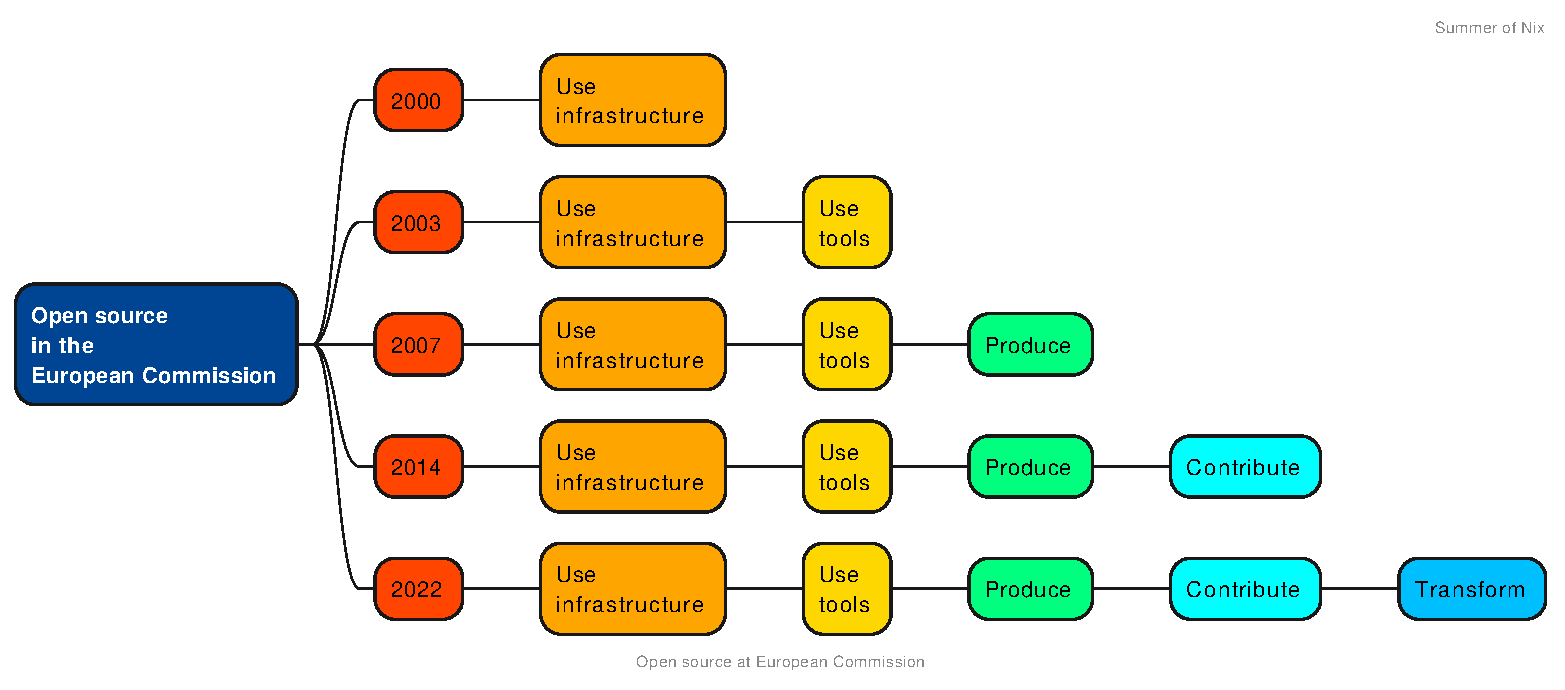
\includegraphics[width=\textwidth,keepaspectratio]{opensource-in-ec}};
      \only<9>{
        \fill [white, opacity=0.9]
        (image.south east) rectangle (image.north west)
        (2.9,-3) rectangle (6.3,-1.75);
      }
    \end{tikzpicture}
  \end{center}

  \note<1>{
    One of the take-aways of this talk would be that the Commission
    recognises the practical value of open source.
  }
  \note<2>{
    Making a talk about Nix already demonstrates how we like this freedom
    to innovate. And how we like sharing these innovations with colleagues
    and with others, such as you - the NixOS community.
  }
  \note<3>{
    But did you know that this is not something new???
  }
  \note<4>{
    Open source and the Commission go back more than twenty years ago.
  }
  \note<5>{
    And over these 20 years, the Commission has grown to appreciate open
    source. To experiment new tools and innovate just like with Nix,
    but also because:
    \begin{itemize}
      \item flexibility,
      \item scalability,
      \item vendor-independence
      \item oftentimes lower costs,
      \item and the list goes on\dots
    \end{itemize}
  }
  \note<6>{
    At EC, DIGIT is the central IT service provider for the Commission. You
    could compare it to 'a ministry of IT'. This is where I work\dots and I can
    tell you that we use open source every where.

    \begin{itemize}
      \item 75\% of our servers runs on Linux,
      \item The PHP language is used for mostly all Commission websites,
      \item NodeJS is used by eUI, a frontend web framework used by all
            internal web applications,
      \item Software developers uses more and more open source tools.
    \end{itemize}
  }
  \note<7>{
    \begin{itemize}
      \item Around 1999, a colleague from JRC created the first building blocks
            of what eventually became Apache, one of the most-popular web
            servers;
      \item In 2007, the Commission published the EUPL license;
      \item And around 2011, Eurostat began sharing some of its tools as open
            source some of its projects;
      \item Since 2019, the ECPHP team - the team I work in - has released a
            dozen of open source projects and materials used within European
            Commission but also in other organisations. We were one of the first
            team doing that.
    \end{itemize}
  }
  \note<8>{
    Over the past two decades, the use of software expanded, from the
    datacenter to Commission desktops - including web browser Firefox,
    media player VLC, LibreOffice, git\dots and so on.
  }
  \note<9>{
    And today, if we had to situate on this graph where we stand, it would
    be here, in the middle of "Contribute and Transform".
  }
  \note<10>{
    That is the reason why you see here in this diagram that there is a
    progression\ldots{}

    \begin{itemize}
      \item from an organisation that consumes open source,
      \item to one that produces its own solutions on top of open source
      \item to one that now wants to become involved in upstream projects
    \end{itemize}
  }
\end{frame}

\subsection{The strategy for the future}

\begin{frame}
  \frametitle{\subsecname}
  \framesubtitle{\secname}

  \begin{columns}[T] % align columns
    \begin{column}{.45\textwidth}
      \begin{center}
        
\includegraphics[width=\textwidth,keepaspectratio]{Infographic_3_oss_strategy-05}
      \end{center}

    \end{column}%
    \hfill%
    \begin{column}{.45\textwidth}

      \begin{itemize}[<+->]
        \item Open source strategy
        \item The strategy impacts the entire organisation
        \item First (public) milestone in September 2022
        \item The idea: a working culture based on the principles of open source
      \end{itemize}

    \end{column}%
  \end{columns}

  \note<1>{
    That is reflected in the open source strategy, officially published in
    2020 which is encouraging the use and reuse of software solutions, knowledge
    and expertise to deliver better European services using open source.

    It also indicates a commitment to support open source developer communities.
  }
  \note<2>{
    Impacting the whole organisation, the strategy led to the creation of a
    dedicated team - the Commission Open Source Programme Office - the OSPO.
  }
  \note<3>{
    On the 16th September in Brno (Czech Republic) we officially unveiled
    code.europa.eu, a public gitlab instance where we aim to share our
    software publicly.
  }
  \note<4>{
    I guess you got big picture, we want open source to be everywhere at EC,
    and not only at DIGIT.
  }
  \note<5>{
    A good example is the cloud framework project 'Simpl', where open source is
    a strict requirement.
  }
  \note<6>{
    But let's check how European Commission is sponsoring Nix projects\dots
  }
\end{frame}

\subsection{Sponsorship}

\begin{frame}
  \frametitle{\subsecname}
  \framesubtitle{\secname}

  \begin{center}
    \begin{tikzpicture}[remember picture, overlay]
      \node[inner sep=0] (image) at (current page.center) {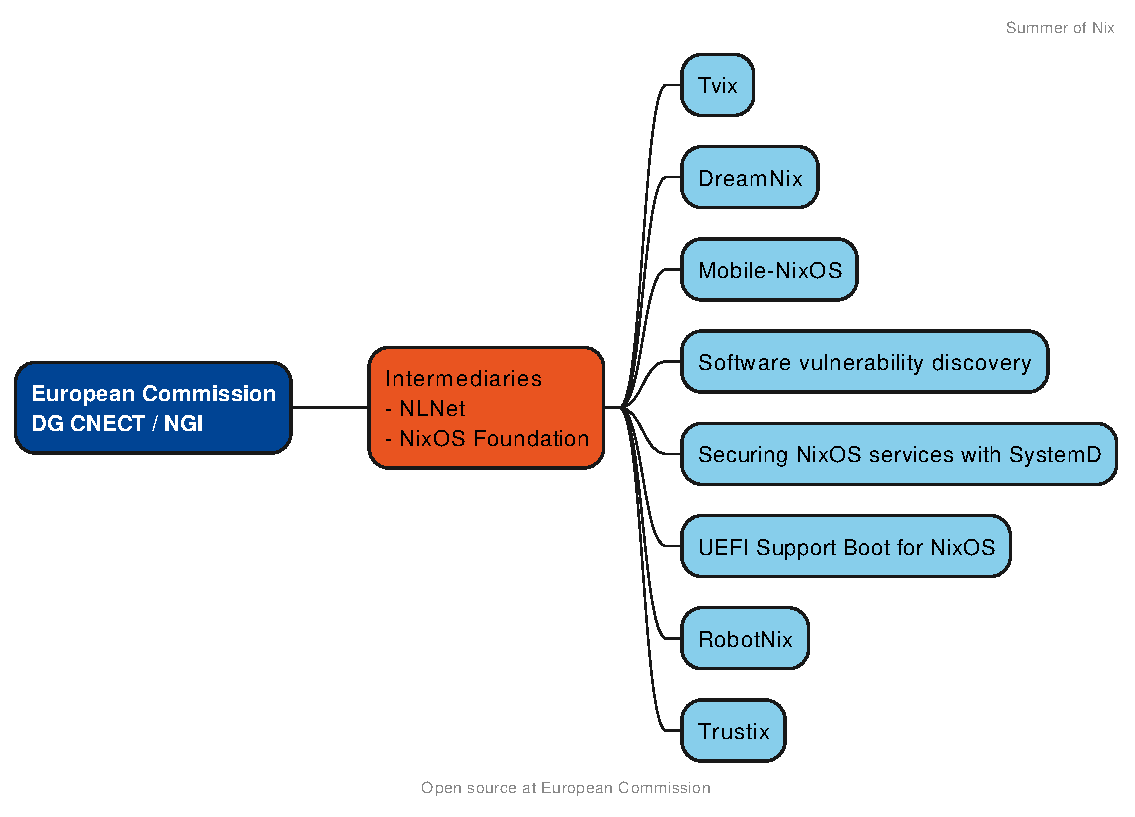
\includegraphics[width=.8\textwidth,keepaspectratio]{sponsoring}};
      \only<1>{
        \fill [white, opacity=0.9]
        (image.south east) rectangle (image.north west)
        (-5.1,-3) rectangle (-2.29,1);
      }
      \only<2>{
        \fill [white, opacity=0.95]
        (image.south east) rectangle (image.north west)
        (-5.1,-3) rectangle (0.30,1);
      }
    \end{tikzpicture}
  \end{center}

  \note<1>{
    About \textpm800 open source projects are funded through DG Connect and NGI.
    (Aside: Connect is like one of the ministries at the EC);

    Examples:
    \begin{itemize}
      \item Wireguard
      \item TOR
      \item F-Droid
      \item OpenPGP
      \item Matrix
      \item Cryptpad
      \item Replicant
      \item Libre and RISC V SOC
    \end{itemize}
  }
  \note<2>{
    European Commission (Connect) has partnerships with NLnet and the NixOS
    Foundation.
  }
  \note<3>{
    It is through those partners / intermediaries that 8 projects related to Nix
    are funded.

    If you would like to get your project funded also, there are open calls and
    submissions are now open till November!
  }
  \note<4>{
    Those projects are:
    \begin{itemize}
      \item Tvix
      \item DreamNix
      \item Mobile-NixOS
      \item Software vulnerability discovery
      \item Securing NixOS services with systemd
      \item UEFI support boot for NixOS
      \item RobotNix
      \item Trustix
    \end{itemize}
  }
  \note<5>{
    Now, let's see how the European Commission is using Nix itself.
    I will begin with some context, and the reasons why it is used.

    And that means you giving you an overview of our environments\dots
  }
\end{frame}

\section{Nix and European Commission}
\subsection{Overview}

\begin{frame}
  \frametitle{\subsecname}
  \framesubtitle{\secname}

  \begin{center}
    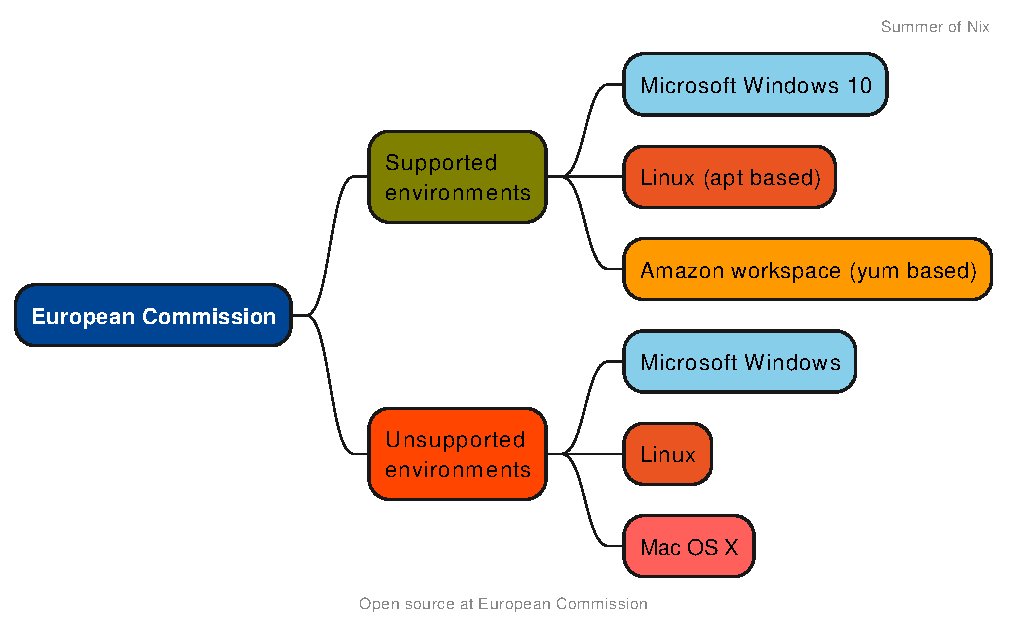
\includegraphics[width=\textwidth,keepaspectratio]{computers}
  \end{center}

  \note<1>{
    In order to reduce the amount of bugs and unforeseen circumstances, we want
    to unify the developer environments.

    Management also wants to reduce the diversity of environments, and
    ensure that we use a development environment which closely match
    what's in production.

    This is quite a challenge since there are a few different operating systems
    in the game as you can see in this graphic.
  }
  \note<2>{
    Some developers uses Microsoft Windows, some Linux on Amazon Workspaces
    using the yum package manager, some are using Linux on their Commission
    laptops which is running on an apt based distro, and some are using
    their own laptops running an arbitrary operating system, Windows, Linux
    or even Mac OS.
  }
  \note<3>{
    In addition to that, some people uses Docker and some others Ansible\dots

    And these tools, while very handy for some specific tasks, are not helping
    at all when it comes to reproducibility and unifying the developers
    development environment.

    Using the proper technology at the proper place is a golden rule.
  }
  \note<4>{
    And while some colleagues were busy exploring new tools to fix all
    aforementioned the issues, I was experimenting with Nix at home.

    So 18 months ago, I got rid of the Linux I was using and started by
    installing NixOS on my own Laptop, then on my backup laptop, then on my
    basement server and finally on my Raspberry running PiHole.

    And you know, since a all these years working with open source, I have in my
    mind the list of open source projects I like the most. First one being
    Blender the 3d suite, this is thanks to that software I ended up using Linux
    so many years ago. Second one is git for its awesomeness and the third
    one is now Nix without hesitation.

    I love this project and its community so much that I've been angry with
    myself to not have discover it earlier. How it is possible ?! What was I
    doing all these years?

    Anyway, enough whining! Here's how I introduced Nix to my colleagues\dots
  }
  \note<5>{
    In the development competency center at DIGIT, the team I work in, I help
    teams and developers of all horizons to be successful in their development,
    promoting the use of best practices, doing live code review,
    proof-of-concept, and abstracting common parts in open source projects.

    One day, a team having issues aligning their development environments.

    They were all using the same Linux flavor, but some of them were not up to
    date, some of them did a major upgrade, some of them were using the bleeding
    edge packages, some others were not able to upgrade for some obscure reasons
    and finally some of them had multiple versions of a software and were unable
    to compile the specific extensions to run their project.

    I guess you see the big picture. It would have been extremely time consuming
    to align everyone\dots and time is money.
  }
  \note<6>{
    And this is how it started, instead of loosing time understanding the
    reasons of all the mess, I decided to use Nix with them for the first time
    \dots and do you know what? They are extremely happy ever since, more
    productive than ever.

    Before going into the details of what I did, let's take a break an list what
    are the requirements of an average developer. This is the same kind of
    question that I asked myself as well.
  }
\end{frame}

\subsection{What does a developer want?}

\begin{frame}
  \frametitle{\subsecname}
  \framesubtitle{\secname}

  \begin{itemize}[<+->]
    \item To have a working development environment, working at anytime of
          the day
    \item Spawning instances of their project quickly
    \item Being aligned with their co-workers
    \item Avoid breaking their laptops
    \item Freedom to use the tool they prefer to do the job
  \end{itemize}

  \note<1>{
    Developers usually wants at anytime of the day, a working development
    environment
  }
  \note<2>{
    Developers usually wants to be able to spawn their projects quickly, as
    many times as they want. They want to quickly focus on what they are good
    at, without adding too much overhead.
  }
  \note<3>{
    Developers usually wants to have the same softwares as their colleagues,
    with the same version. It's easier to reproduce an issue in case of
    bugs.
  }
  \note<4>{
    Developers usually wants to avoid breaking their laptop when they have
    to install different or multiple versions of a particular software.
  }
  \note<5>{
    An happy and productive developer is a developer who uses its own tool.
    I guess there's no need to explain further, we all know what it means.

    A real life example would be me. Using the EC Linux laptop felt like a
    burden because I couldn't reproduce quickly and easily my usual development
    environment\dots

    Spoiler alert, I now use exclusively that laptop since I discovered Nix!
  }
  \note<6>{
    Given this, I ran a series of experiments with my colleagues, iterating over
    and over again until we reached some sort of stability and ease of use with
    Nix.
  }
\end{frame}

\subsection{What are we experimenting?}

\begin{frame}
  \frametitle{\subsecname}
  \framesubtitle{\secname}

  \begin{itemize}[<+->]
    \item Nix flakes
    \item nix-direnv
    \item home-manager \textcolor{fg!25}{(publicly available @ \href{https://code.europa.eu/ecphp/devs-profile}{code.europa.eu})}
    \item Servers running NixOS
  \end{itemize}

  \note<1>{
    By shipping a custom Nix flake per project, developers are able to
    customize their development environment at will.

    A simple example is this open source \LaTeX\ presentation which is hosted on
    code.europa.eu with a flake file containing the required dependencies to
    build and contribute to it without worries.
  }
  \note<2>{
    I use direnv and it's brother nix-direnv to load software dependencies
    without typing any single command. This is fast, this is handy, this is
    a really unique tool that unleash it's full potential when it is used
    with Nix.
  }
  \note<3>{
    I also created a trivial home-manager profile setting up a custom shell
    with some carefully chosen plugins, custom aliases and nix-direnv
    integration.

    Thanks to that, it reduces the amount of time a developer needs to spend
    setting up it's workstation, because this profile set everything up with one
    single command and a few seconds.
  }
  \note<4>{
    Very recently, in the OpenSource Project Office team we wanted to host
    our own instance of a note service, and we ended up setting up a bunch
    of servers. One reverse proxy, one HedgeDoc instance and some others.
    All managed by a single flake file and guess what\dots, we deploy on
    Fridays without any worries!

    While setting up our ``Infrastructure as Code'', we contributed to NixOS by
    creating pull requests to fix minor issues we had.
  }
  \note<5>{
    And just like you most probably know, the road to success is never a
    straight line\dots

    The problems I have with the adoption of Nix could be summarized in one
    quote from Albert Einstein, here it is\dots
  }
\end{frame}

\begin{frame}[plain]
  \begin{quote}
    The world as we have created it is a process of our thinking.\\It cannot be
    changed without changing our thinking.
    \par\nobreak\smallskip\hfill ~---~ Albert Einstein
  \end{quote}

  \note<1>{
    <read the quote>\dots

    <make a pause>\dots

    This is something we should always have in mind.

    And Mr Einstein was right, and more than a hundred years later, he still
    is right\dots despite the efforts that are made to try to break Relativity.
  }

  \note<2>{
    It's often the same pattern when something new needs to be introduced\dots

    Remember that people feared electricity when it was invented.
    There will always be ignorance, and ignorance leads to fear.

    And it's the same when it comes to Nix at European Commission.
  }

  \note<2>{
    All of this to introduce my next slide which is about the pain points
    introducing Nix at European Commission.
  }
\end{frame}

\subsection{Which problems are we facing?}

\begin{frame}
  \frametitle{\subsecname}
  \framesubtitle{\secname}

  \begin{itemize}[<+->]
    \item The fear of the unknown,
    \item The use of experimental features,
    \item The programming language,
    \item The documentation.
  \end{itemize}

  \note<1>{
    Every new piece of software fixes issues but also brings in a couple of new
    issues. Nix is quite new at E.C. and people are sometimes a bit
    reluctant to use something they never heard of\dots yet.
  }
  \note<2>{
    Flake is a feature that has been introduced in November 2021 and nowadays it
    is still considered as experimental.

    Given that, asking to such an institution to use an experimental feature in
    their day to day work might be a little bit more difficult.
  }
  \note<3>{
    Learning the Nix programming language can be tedious for developers who
    never used functional programming at all.

    But this might not be true since last week with the new tutorial that has
    been published on nix.dev (https://nix.dev/tutorials/nix-language).
  }
  \note<4>{
    About documentation, there are still a lot of work to be done.

    This is the reason why there is a new documentation team in place in the
    community, they are in charge of "flattening the curve". That new Nix
    tutorial is actually their first outcome and many more are coming, I can't
    wait to see that.
  }
\end{frame}

\subsection{What's next?}

\begin{frame}
  \frametitle{\subsecname}
  \framesubtitle{\secname}

  \begin{itemize}[<+->]
    \item Continue to experiment and evaluate Nix,
    \item Find other candidates for testing,
    \item Improve our custom development profile,
    \item Ship a \texttt{flake.nix} for each project,
    \item Contribute to the community.
  \end{itemize}

  \note<1>{
    The idea is obviously to continue experimenting with Nix, testing things and
    see how it could be adopted more broadly.

    I believe that the issues related to the fear of unknown will disappear with
    time.

    The flake feature is about to loose it's experimental flag, this is going to
    encourage more and more people to join in.

    The programming language? This is like any other language, as long as we
    have a good documentation, we can learn it correctly.
  }
  \note<2>{
    In my team, the development profile will be improved and its documentation
    as well. This idea would be to tell about this profile to other teams and
    show how it can be used in conjunction of what's already existing.
  }
  \note<3>{
    I wish I could ship a flake file per project to reduce to almost zero the
    amount of time new developers need to spend to setup their environment.
    This is already the case for all the open source projects in my team, but it
    would be a big plus if it could be done on other projects by default.
  }
  \note<4>{
    About contributing, we already contributed back to NixOS with a couple of
    pull requests. The idea is to continue to work with this mindset of
    openness, re-usability and sharing.
  }
  \note<5>{
    This last and positive slide conclude my presentation, feel free to ask your
    questions\dots
  }
\end{frame}

% \begin{frame}[t]{Title of frame}
%   \begin{columns}[T,onlytextwidth]
%     \begin{column}{.4\textwidth}
%       \begin{minipage}{\textwidth}
%         \begin{figure}
%           \includegraphics[width=\textwidth]{example-image}
%         \end{figure}
%         \footnotetext{Figure left top}
%       \end{minipage}
%       \begin{onlyenv}<3>
%         \begin{minipage}{\textwidth}
%           \begin{figure}
%             \includegraphics[width=\textwidth]{example-image}
%           \end{figure}
%           \footnotetext{Figure left bottom}
%         \end{minipage}
%       \end{onlyenv}
%     \end{column}
%     \begin{column}{.4\textwidth}
%       \begin{onlyenv}<2->
%         \begin{minipage}{\textwidth}
%           \begin{figure}
%             \includegraphics[width=\textwidth, height=.77\textheight]{example-image}
%           \end{figure}
%           \footnotetext{Figure right}
%         \end{minipage}
%       \end{onlyenv}
%     \end{column}
%   \end{columns}
% \end{frame}

% \begin{frame}
%   \begin{columns}
%     \column{\paperwidth}
%     \includegraphics[width=\the\paperwidth, height=.5\paperheight]{example-image}
%     \begin{tikzpicture}
%       \node[shape=rectangle, text opacity=1,minimum height=.5\paperheight, minimum width=\paperwidth, anchor=south]{
%         BODY
%       };
%     \end{tikzpicture}
%   \end{columns}
% \end{frame}

% \begin{frame}
%   \begin{columns}
%     \column{.5\paperwidth}
%     \includegraphics[width=.5\paperwidth, height=\paperheight]{example-image}
%     \column{.5\paperwidth}
%     \begin{tikzpicture}
%       \node[shape=rectangle, text opacity=1,minimum height=\paperheight, minimum width=.5\paperwidth, anchor=east]{
%         BODY
%       };
%     \end{tikzpicture}
%   \end{columns}
% \end{frame}

\end{document}
